\chapter{基礎方程式}
本章では油圧システムについてのモデリングの導出を行う.
対象とする油圧システムの模式図は図で表され,4ポートサーボバルブと片ロッドシリンダが接続されているものとなる.
このサーボバルブとシリンダについてJalaliら\cite{jelali2012hydraulic} に従いながら第一原理に基づき基礎方程式の記述を行う.
\begin{figure}[t]
    \centering
        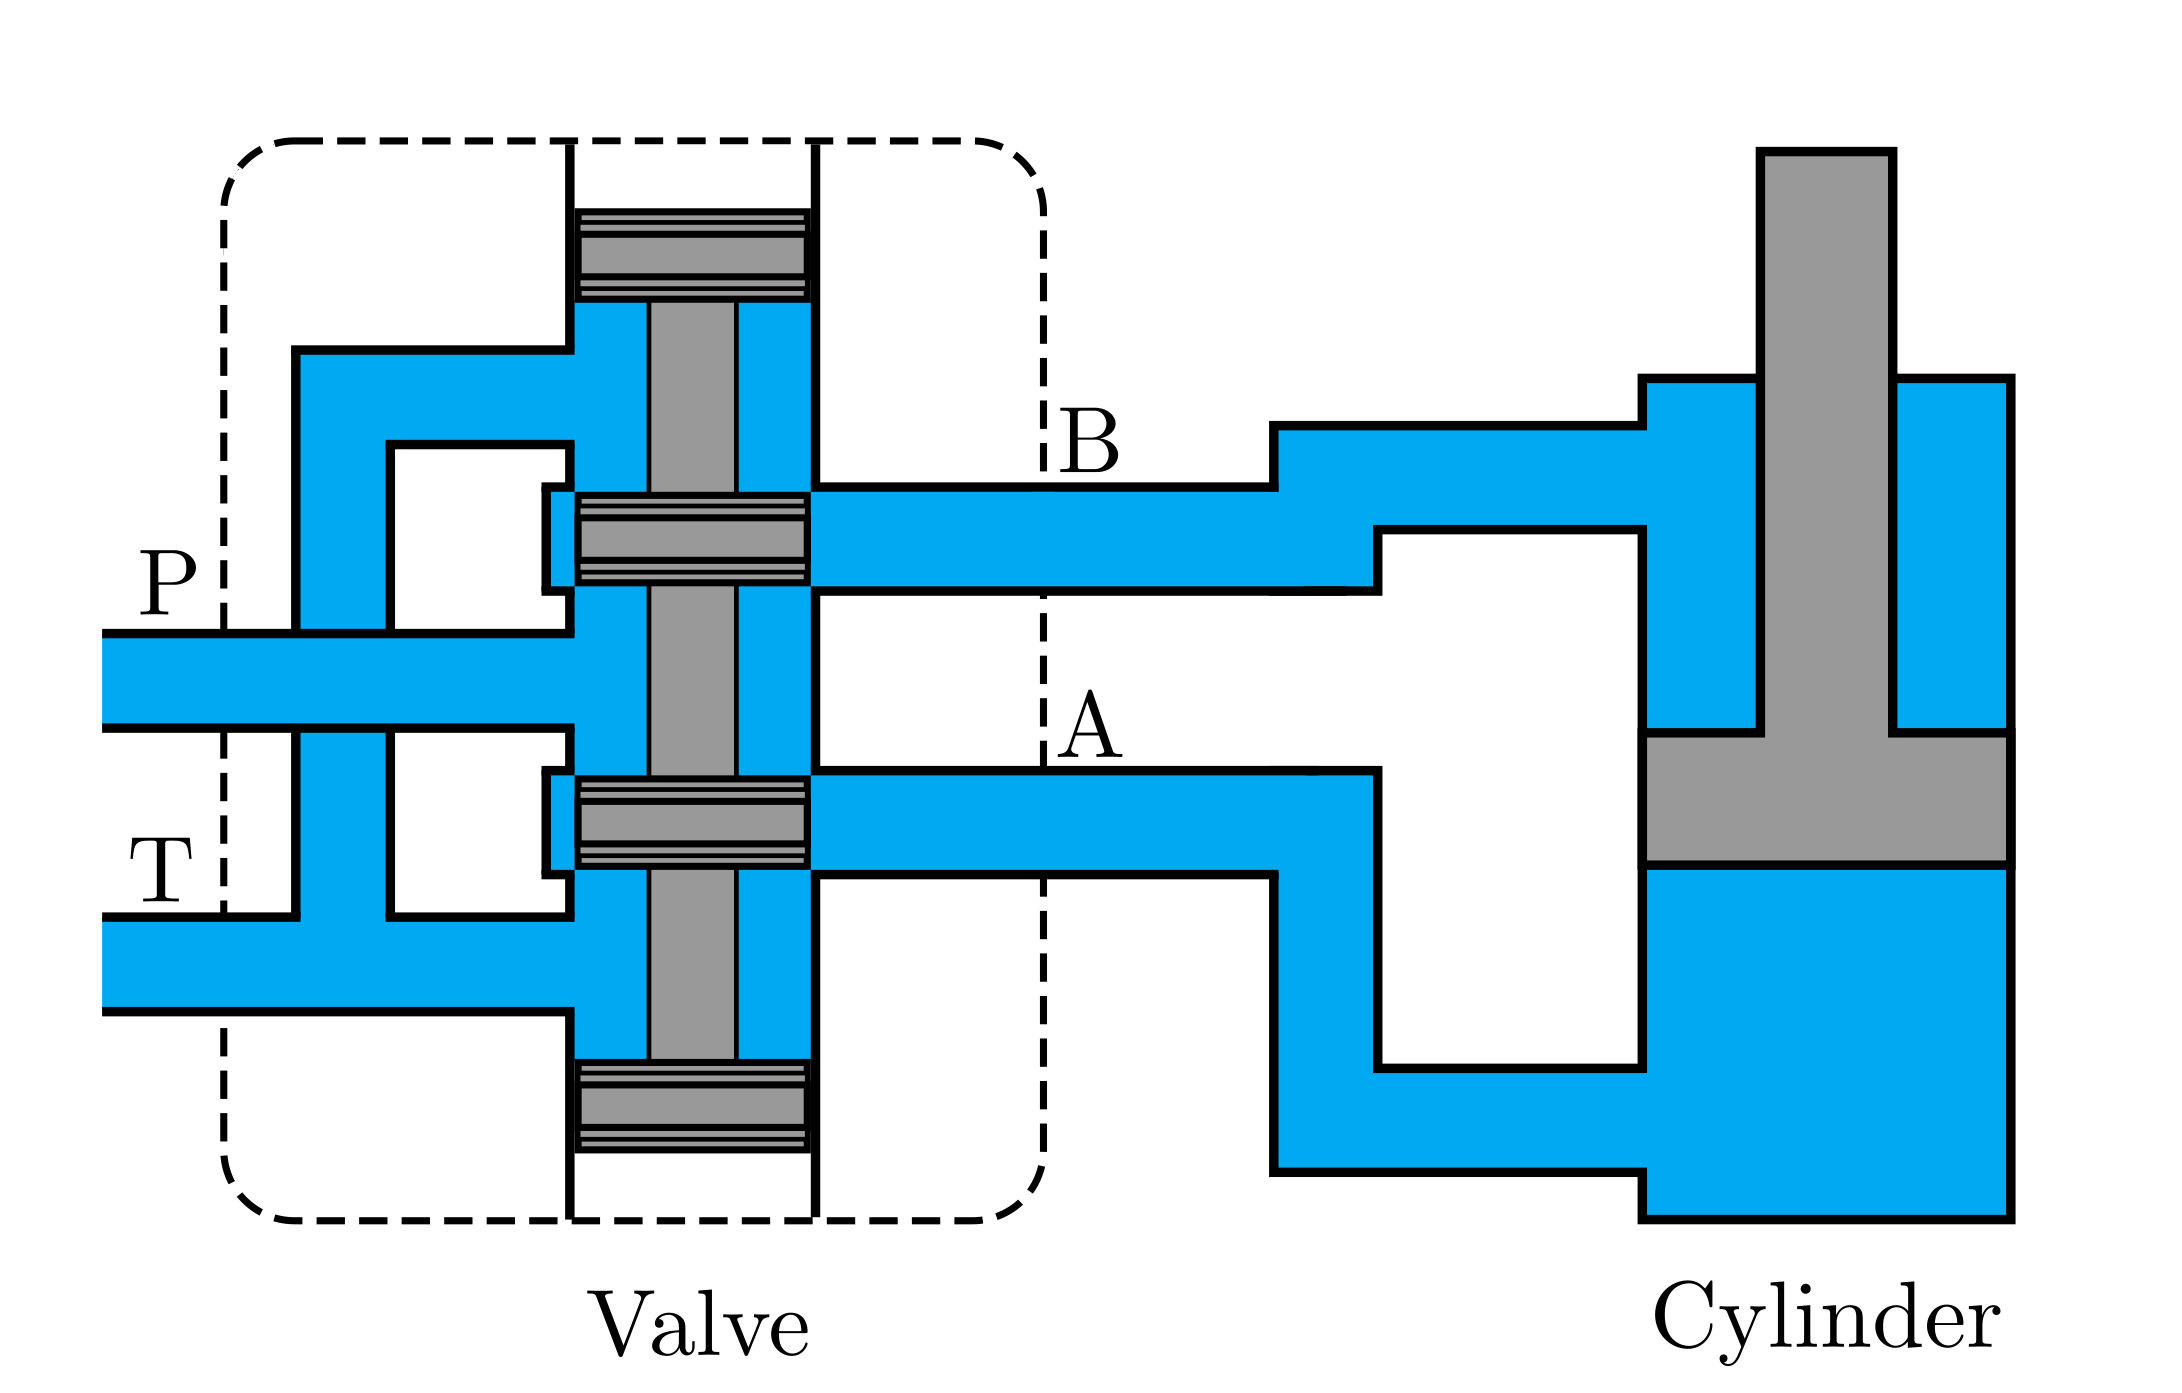
\includegraphics[keepaspectratio, scale=1.0]{contents/基礎方程式/figure/valve-cylinder.png}
        \caption{サーボバルブの図}
        \label{fig:figlabel}
\end{figure}

\section{サーボバルブ}
\subsection{サーボバルブの各部名称とパラメータ}
ここでは4ポート式サーボバルブの各部名称,および変数設定について述べる.
\begin{figure}[t]
    \centering
        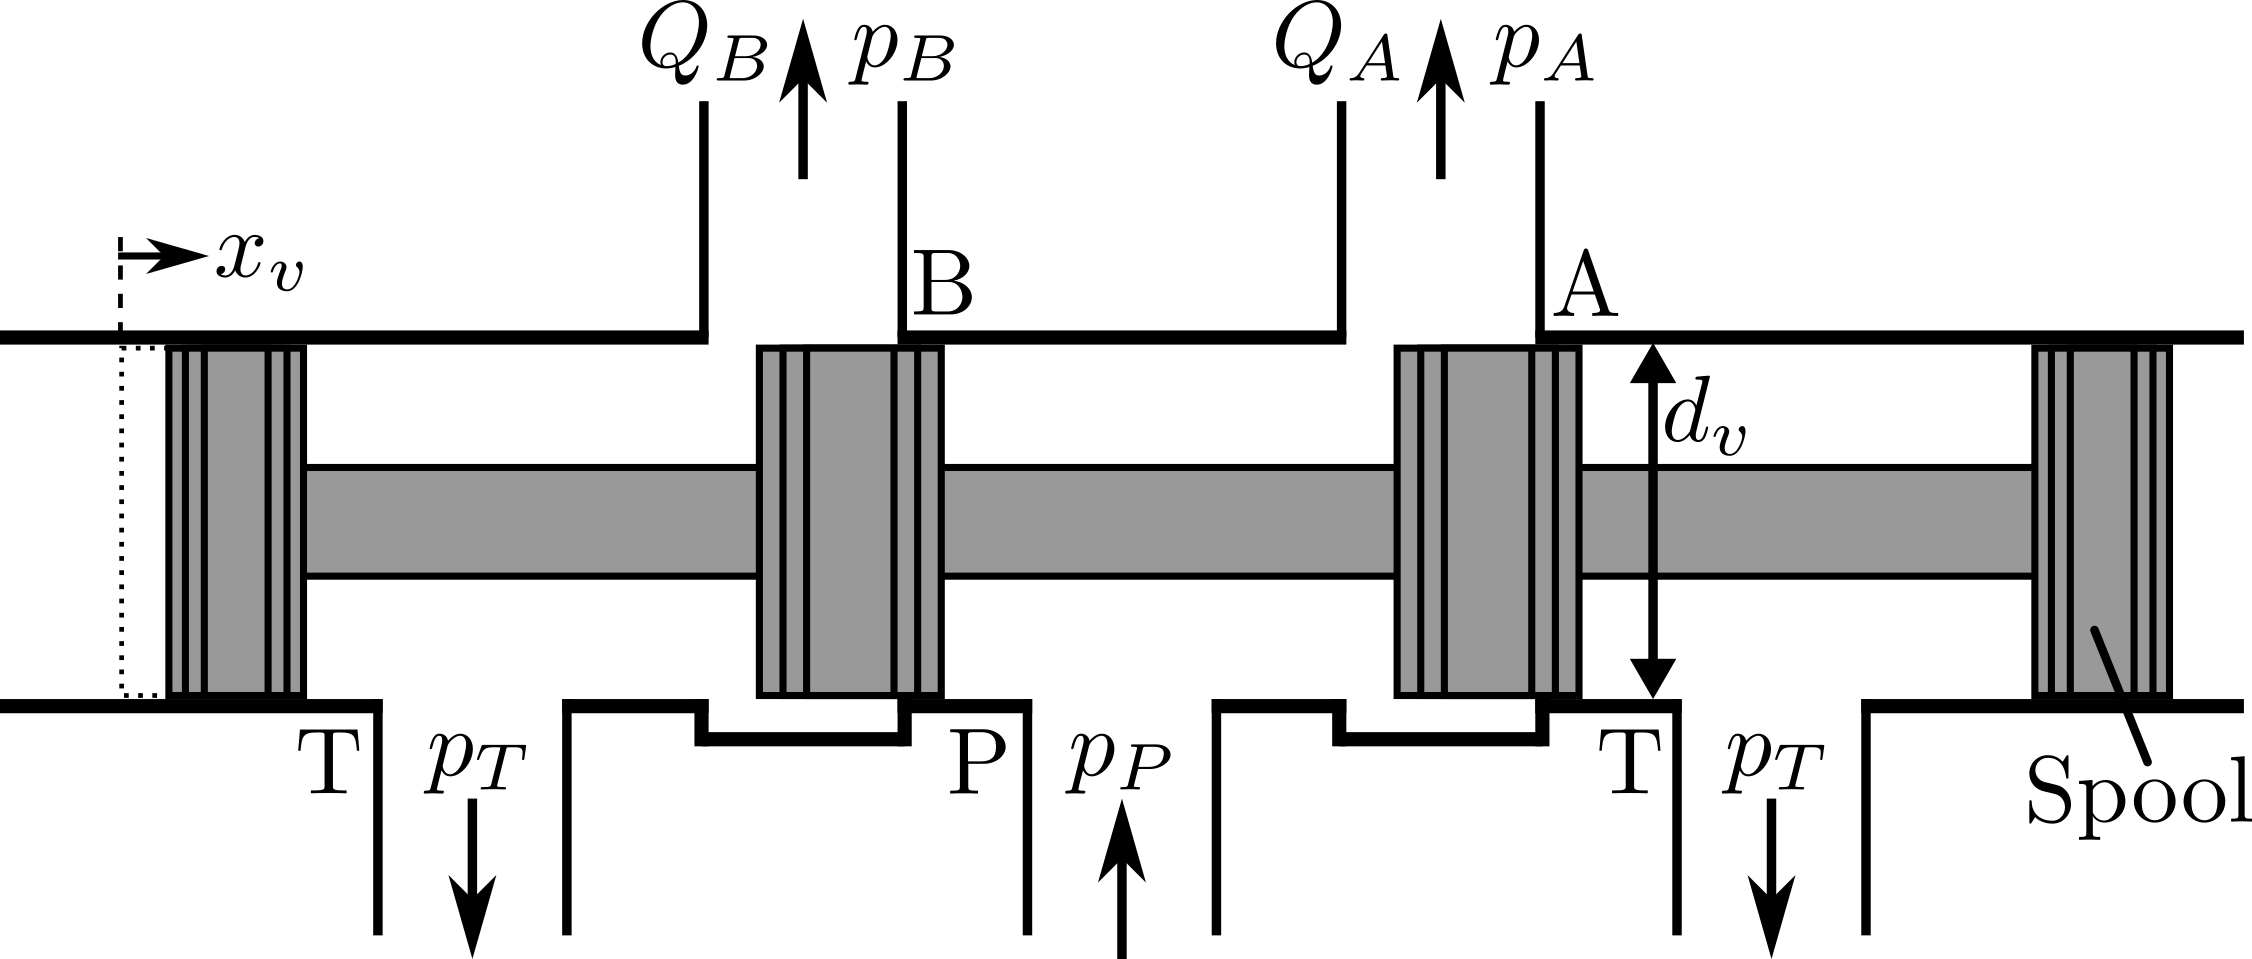
\includegraphics[keepaspectratio, scale=1.0]{contents/基礎方程式/figure/valve.png}
        \caption{サーボバルブの図}
        \label{fig:figlabel}
\end{figure}
\subsection{サーボバルブを通過する流量}
作動流体がサーボバルブを通過する流れは,オリフィス流れであるとみなされる.
オリフィスを通過する流量$Q$は,一般に
\begin{equation}
    Q = \alpha_d A \sqrt{\frac{2}{\rho}\Delta p}
    \label{eq:orifice_flow}
\end{equation}
と表される.
ここで,$\alpha_d$は流出係数(discharge coefficient),$A$は流体の断面積,$\rho$は流体の密度,$\Delta p$はオリフィス前後の十分離れた場所における流体の圧力の差である.
サーボバルブにおけるスプールの中立点からの変位を$x_v$とし,流体の流れる方向を考慮すると,\eqnname\ref{eq:orifice_flow}は
\begin{align}
    \label{eq:orifice_valve}
    Q(x_v,\Delta p)&= c_vx_v\mathrm{sign}(\Delta p)\sqrt{\Delta p}\\
    c_v &= \pi d_v \alpha_d\sqrt{\frac{2}{\rho}}
\end{align}
となる.
$\mathrm{sign}(\cdot)$はシグナム関数であり,以下で定義される.
\begin{align}
    \label{eq:function_sign}
    \mathrm{sign}(x) = 
    \begin{cases}
        1~&(\mathrm{if}~x>0)\\
        0~&(\mathrm{if}~x=0)\\
        -1~&(\mathrm{if}~x<0)
    \end{cases}
\end{align}

サーボバルブの制御ポートAから吐き出される流量$Q_A$は,「供給ポートPから制御ポートAへ流れる流量$Q_{PA}$」と「制御ポートAから戻りポートTへの流量$Q_{AT}$」の差分で表される.
供給ポートPから制御ポートAへ流れるときのスプール変位$x_v$を正とすると,このときには$Q_{AT}$は0となる.
逆に$x_v$が負のときには$Q_{PA}$は0となる.
これらをまとめると,$Q_A$は,\eqnname\ref{eq:orifice_valve}も考慮すると,
\begin{align}
    \notag
    \label{eq:flow_QA}
    Q_A =& Q_{PA}- Q_{AT} \\ \notag
    =&c_{v_{PA}}\mathrm{sg}(x_v)\mathrm{sign}(p_P-p_A)\sqrt{|p_P-p_A|} \\ 
    &- c_{v_{AT}}\mathrm{sg}(-x_v)\mathrm{sign}(p_A-p_T)\sqrt{|p_A-p_T|}
\end{align}
となる.
同様に,制御ポートBへ吐き出される流量$Q_B$は,向きが$Q_A$と逆になることに注意して
\begin{align}
    \label{eq:flow_QB}
    \notag
    Q_B =& Q_{PB}- Q_{BT} \\ \notag
    =&-c_{v_{PB}}\mathrm{sg}(-x_v)\mathrm{sign}(p_P-p_B)\sqrt{|p_P-p_B|} \\ 
    &+ c_{v_{BT}}\mathrm{sg}(x_v)\mathrm{sign}(p_B-p_T)\sqrt{|p_B-p_T|}
\end{align}
となる.
$\mathrm{sg}(\cdot)$は,
\begin{align}
    \label{eq:function_sg}
    \mathrm{sg}(x) = 
    \begin{cases}
        x&(\mathrm{if}~x>0)\\
        0&(\mathrm{if}~x\leq0)\\
    \end{cases}
\end{align}
で定義される関数である.

\subsection{サーボバルブの動特性}
サーボバルブへの指令電圧入力$u_v$とスプール変位$x_v$の関係は,周波数応答などから\eqnname\ref{eq:valve_freq}に示す二次系の運動方程式で近似して表すことができる.
\begin{equation}
    \label{eq:valve_freq}
    \frac{1}{\omega_v^2}\ddot{x}_v^* + \frac{2D_v}{\omega_v}\dot{x}_v^* + x_v^* + f_{hs}\mathrm{sign}(\dot{x}_v^*) = K_v u_v^*
\end{equation}
なお,$u_v^*$や$x_v^*$などはそれぞれ入力電圧の最大値$u_{v,max}$,スプール変位の最大値$x_{v,max}$で除して正規化されたものであり,以下の\eqnname\ref{eq:normalize_u}から\eqnname\ref{eq:normalize_xv}で定義される.
\begin{align}
    \label{eq:normalize_u}
    u_v^* &= \frac{u_v}{u_{v,max}}\\
    \label{eq:normalize_xv}
    x_v^* = \frac{x_v}{x_{v,max}}~,~\dot{x}_v^* &= \frac{\dot{x}_v}{x_{v,max}}~,~\ddot{x}_v^* = \frac{\ddot{x}_v}{x_{v,max}}
\end{align}
また,\eqnname\ref{eq:valve_freq}において$K_v$はバルブのゲイン,$\omega_v$は固有角振動数,$D_v$は粘性係数,$f_{hs}$はバルブのヒステリシスや応答感度を表す関数である.
\section{油圧シリンダー}
油圧シリンダー内の作動流体についてモデル化する.
流体の質量保存則は\eqnname\ref{eq:situryouhozon}である.
\begin{equation}
    \label{eq:situryouhozon}
    \Sigma m_{in}-\Sigma m_{out} = \frac{\mathrm{d}(\rho V)}{\mathrm{d}t} = \rho \dot{V}+\dot{\rho}V
\end{equation}
$\rho$は流体の密度であり,圧縮性流体においてはその表現方法は文献により様々であるが,本論文では以下の\eqnname\ref{eq:rho_teigi}で定義される$\rho$を採用する.
\begin{equation}
    \label{eq:rho_teigi}
    \rho = \rho_i + \frac{\rho_i}{E(p)}p
\end{equation}
ここで$\rho_i$は圧力が0のときの密度,$E(p)$はバルクモジュールである,$p$は流体の圧力である.

\section{モデルの線形化とラプラス変換}

\section{運動方程式と摩擦のモデル}